%%%%%%%%%%%%%%%%%%%%%%%%%%%%%%%%%%%%%%%%%
% Beamer Presentation
% LaTeX Template
% Version 1.0 (10/11/12)
%
% This template has been downloaded from:
% http://www.LaTeXTemplates.com
%
% License:
% CC BY-NC-SA 3.0 (http://creativecommons.org/licenses/by-nc-sa/3.0/)
%
%%%%%%%%%%%%%%%%%%%%%%%%%%%%%%%%%%%%%%%%%

%----------------------------------------------------------------------------------------
%	PACKAGES AND THEMES
%----------------------------------------------------------------------------------------

\documentclass{beamer}

\usetheme{Antibes}
\usecolortheme{seagull}

\usepackage{graphicx} % Allows including images
\usepackage{booktabs} % Allows the use of \toprule, \midrule and \bottomrule in tables

\usepackage{listings}

\definecolor{codegreen}{rgb}{0,0.6,0}
\definecolor{codegray}{rgb}{0.5,0.5,0.5}
\definecolor{codepurple}{rgb}{0.58,0,0.82}
\definecolor{backcolour}{rgb}{0.95,0.95,0.92}



%----------------------------------------------------------------------------------------
%	TITLE PAGE
%----------------------------------------------------------------------------------------

\title[Domain Driven Design in Action]{Domain Driven Design in Action}

\author{Mohamed Sweelam} 
\institute[msweelam.carrd.co]
{
	Software Engineer \\
	\medskip
	\textit{md.sweelam@gmail.com}
}
\date{\today}


\usefonttheme{professionalfonts}
\begin{document}
	\begin{frame}
	\titlepage
\end{frame}

\begin{frame}
	\frametitle{Objectives} 
		\begin{enumerate}
			\item<1-> \large {Provide good Arabic content for the topic}
			\item<2-> \large {Overview of DDD and Deep Dive in Microservices}
			\item<3-> \large {Move step forwards towards recent cloud tools}
			\item<4-> \large {Leave your fear, and let's do it}
		\end{enumerate}
\end{frame}

\begin{frame}
\frametitle{Table of Contents} 
	\scriptsize
	\tableofcontents
\end{frame}


\section{Strategic Design}
	\subsection {Introduction to Software Architecture}
		\begin{frame}
			\frametitle{Definition}
				\begin{block}{Monolithic}
					A monolithic application is self-contained, and independent from other computing applications. The design philosophy is that the application is responsible not just for a particular task, but can perform every step needed to complete a particular function.
				\end{block}
			
			\vspace{5mm}
			\begin{block}{Microservices}
				Microservices is a software development technique that arranges an application as a collection of loosely coupled services. 
			\end{block}
			
			\vspace{10mm}
			\tiny{https://en.wikipedia.org/wiki/Monolithic\_application}\\
			\tiny{https://en.wikipedia.org/wiki/Microservices}		
		\end{frame}
		
		
	\subsection {Introduction to Domain Driven Design}
		\begin{frame}
			\scriptsize
			Domain-Driven Design(DDD) is a collection of principles and patterns that help developers craft elegant object systems.
			\begin{figure}[h]
				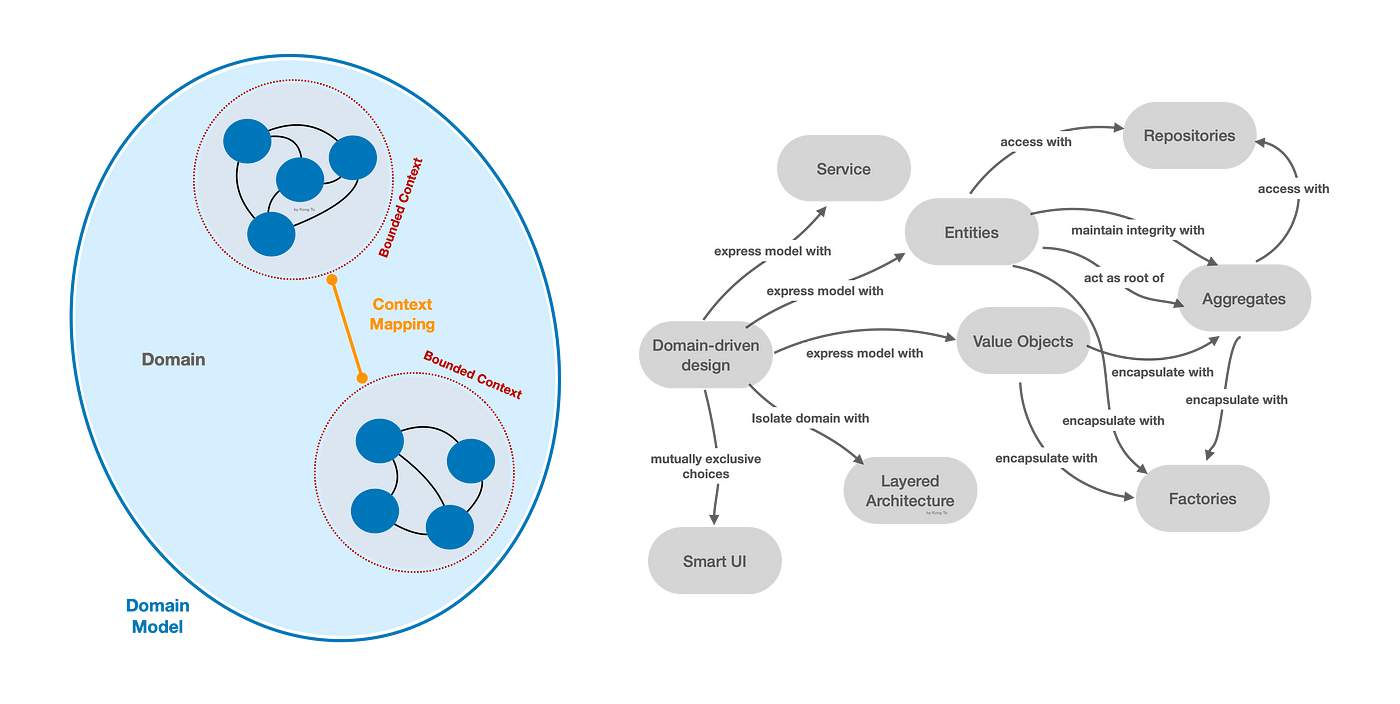
\includegraphics[width=0.8\linewidth , height=60mm]{img/domain-driven-arch.png}
				\caption{DDD Map}
			\end{figure}
		
		\end{frame}
	
	\subsection {Strategic Design and Domain Crunching}	
		\begin{frame}
			\begin{figure}[h]
				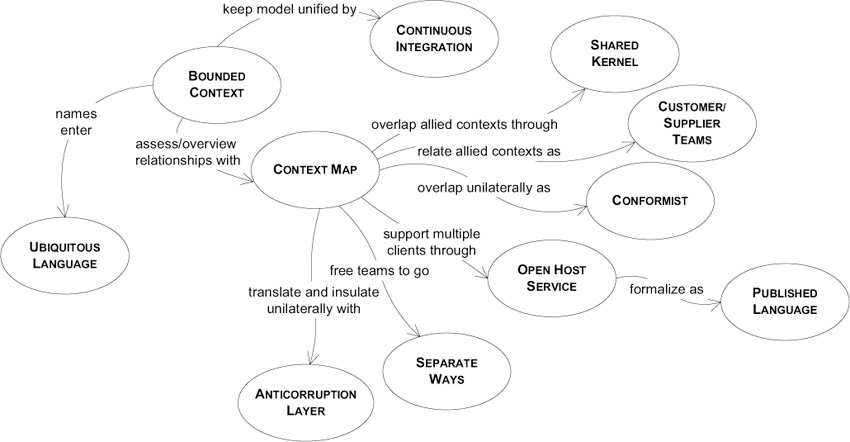
\includegraphics[width=0.8\linewidth , height=60mm]{img/strategic-map.png}
				\caption{Strategic Design Map}
			\end{figure}
		\end{frame}
	
	\subsection {Ubiquitous Language}		
		\begin{frame}
			\begin{figure}[h]
				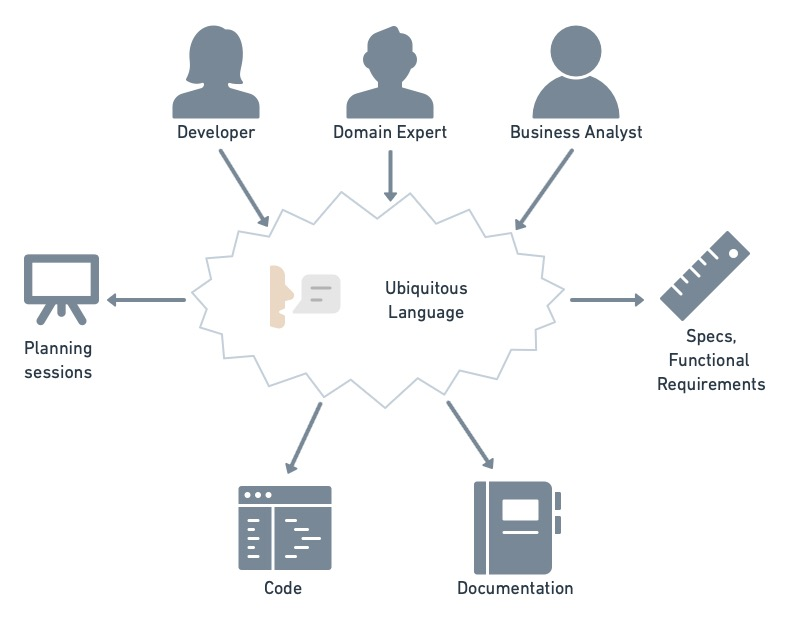
\includegraphics[width=0.8\linewidth , height=60mm]{img/ubiquitous-language.png}
				\caption{All Speak The Same Language "Ubiquitous Language"}
			\end{figure}
		\end{frame}
	
	\subsection {Context Mapping}
		\begin{frame}
		---
		\end{frame}
		
\section{Tactical Design}
	\subsection {Entities vs Value Objects}
		\begin{frame}
		---
		\end{frame}

	\subsection {Aggregate and Aggregate Roots}
		\begin{frame}
		---
		\end{frame}

	\subsection {Repositories}
		\begin{frame}
		---
		\end{frame}

	\subsection {Domain Services}
		\begin{frame}
		---
		\end{frame}

	\subsection {Factories}
		\begin{frame}
		---
		\end{frame}
	
		
\section {Microservices Core Principles}
	
	\subsection	{Why Microservices?}
		\begin{frame}
			\frametitle{Why Microservices?}
				\begin{enumerate}
					\item<1-> Unit design
						\begin{itemize}
							\item \scriptsize {The application consists of loosely coupled services}. 
							\item \scriptsize {Each service supports a single business task}.
						\end{itemize}
					\item<2-> Flexibility
						\begin{itemize}
							\item \scriptsize {Each microservice can be developed using a programming language and framework that best suits}.
						\end{itemize}
					\item<3-> Maintainability
						\begin{itemize}
							\item \scriptsize {Simple, focused, and independent. So the application is easier to maintain}.
						\end{itemize}
					\item<4-> Resiliency
						\begin{itemize}
							\item \scriptsize {The application functionality is distributed across multiple services}. 
							\item \scriptsize {If a microservice fails, the functionality offered by the others continues to be available}.
						\end{itemize}
					\item<5-> Scalability
						\begin{itemize}
							\item \scriptsize {Each microservice can be scaled independently of the other services}.
						\end{itemize}
				\end{enumerate}
		\end{frame}

	\subsection {Microservices vs Monolithic}
		\begin{frame}
			\frametitle{Microservices vs Monolithic}
				\begin{figure}[h]
					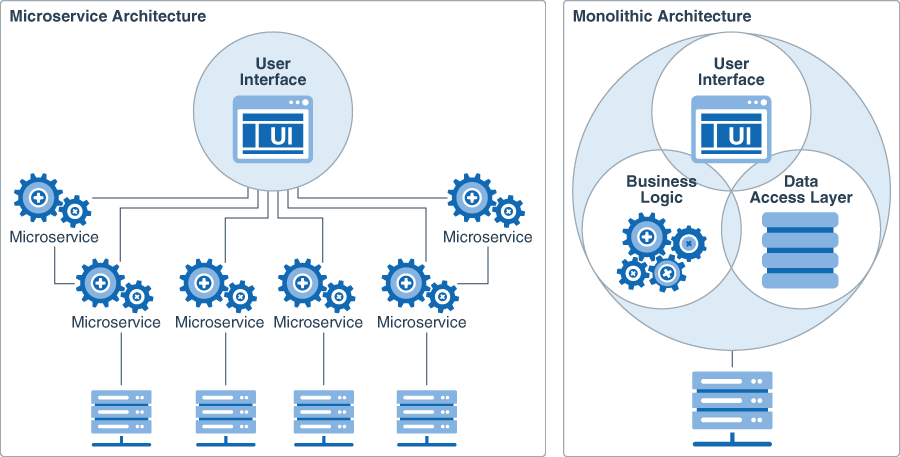
\includegraphics[width=0.8\linewidth]{img/monolithic_vs_microservice.png}
					\caption{mivroservices vs monolithic}
				\end{figure}
				
				
				\tiny{https://docs.oracle.com/en/solutions/learn-architect-microservice/index.html}		
		\end{frame}

		\begin{frame}
			\frametitle{Closer Look}
				\begin{figure}[h]
					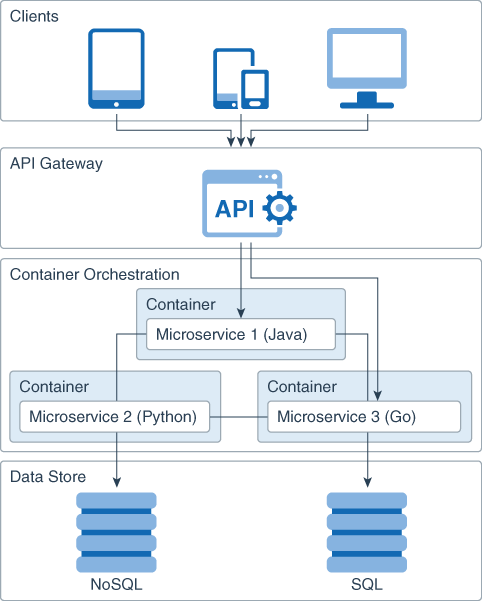
\includegraphics[width=55mm, height=55mm, scale=1]{img/microservice_architecture.png}
					\caption{Microservices In Depth}
				\end{figure}
				
				
				\tiny{https://docs.oracle.com/en/solutions/learn-architect-microservice/index.html}	
		\end{frame}
	
	\subsection {Microservices Architecture}
		\begin{frame}
			\frametitle{Microservices Architecture}
				\begin{figure}[h]
					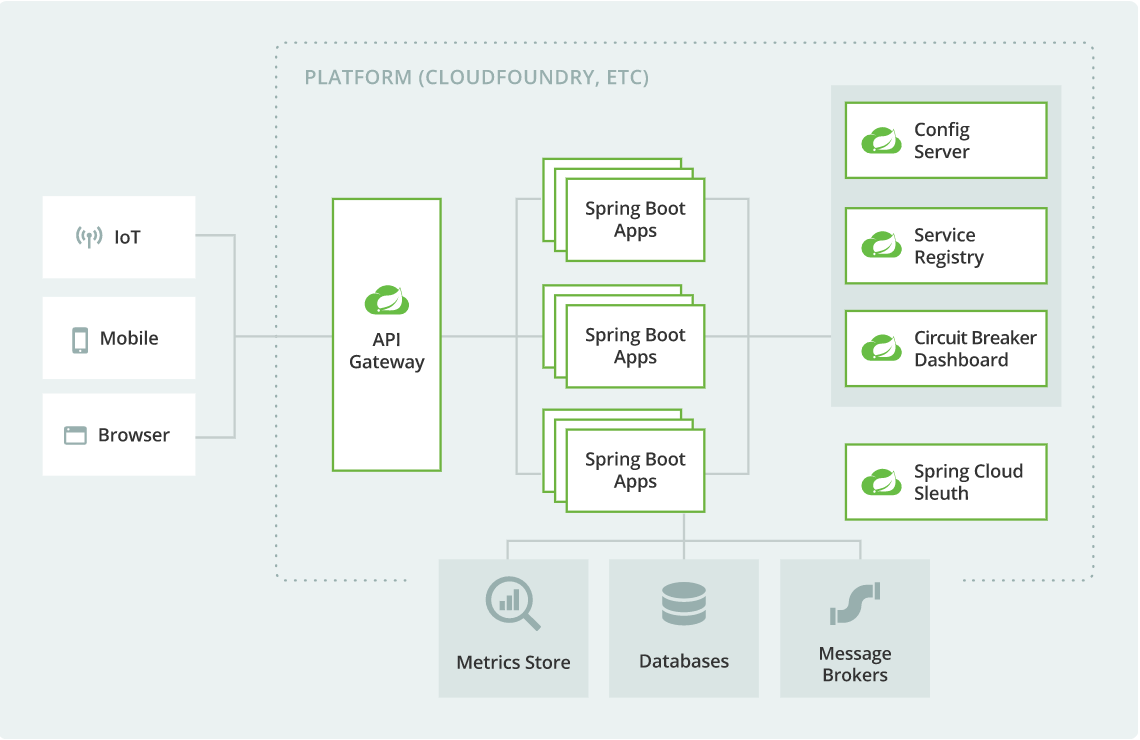
\includegraphics[width=100mm, scale=2]{img/microservice-diagrame.png}
					\caption{Microservices with Spring Cloud}
				\end{figure}\vspace{20mm}

				\tiny{https://spring.io/microservices}	
		\end{frame}
	
		\begin{frame}
			\frametitle{Microservice characteristics}
				\begin{columns}[c]
					\column{.40\textwidth} 
						\hspace{2mm} \textbf {Single Responsibility}
						\begin{itemize}
							\item Business Boundary
							\item Function Boundary
						\end{itemize}
					
					\column{.70\textwidth} % Right column and width
						\begin{figure}[h]
							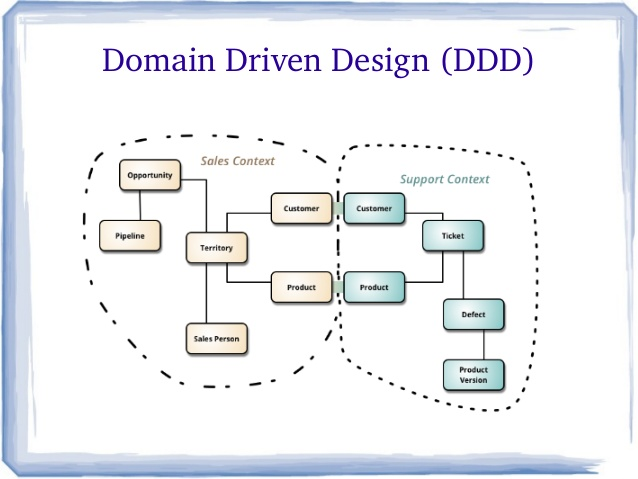
\includegraphics[width=70mm, height=50mm, scale=1]{img/ddd.jpg}
						\end{figure}\vspace{1mm}
				\end{columns}
			
			\vspace{10mm}
			\tiny{https://martinfowler.com/bliki/BoundedContext.html}
		\end{frame}

		
	\subsection {Communication Design}
		\begin{frame}[label=cd]
			\frametitle{Communication Design}
				\begin{block} {HTTP communication}
					Also known as \textbf{Synchronous communication}, the calls between services is a viable option for \textbf{service-to-service} via REST API.
				\end{block}
				
				\vspace{2mm}
				\begin{block} {Message communication}
					Also known as \textbf{Asynchronous communication}, the services push messages to a message broker that other services subscribe to.
				\end{block}
			
			\vspace{2mm}
			\begin{block} {Event-driven communication}
				Another type of \textbf{Asynchronous communication}, the services does not need to know the common message structure. Communication between services takes place via events that individual services produce.
			\end{block}
		
		\vspace{5mm}
		\tiny {https://blog.logrocket.com/methods-for-microservice-communication}
		\end{frame}
	
	\begin{frame}
		\frametitle{HTTP communication}
			\begin{figure}[h]
				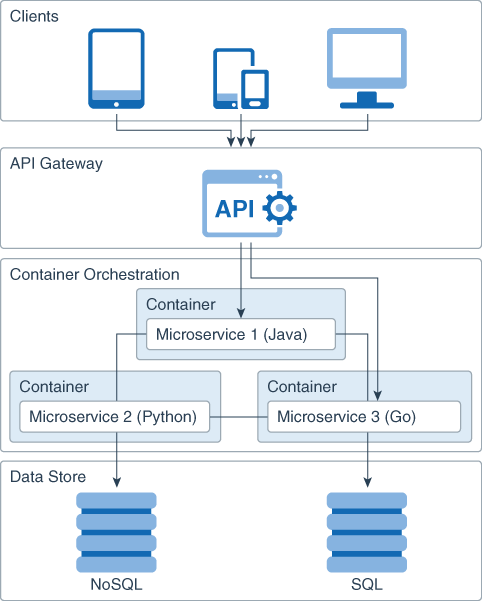
\includegraphics[width=55mm, height=60mm scale=1]{img/microservice_architecture.png}
				\caption{Service to Service Calls}
			\end{figure}
	\end{frame}
	
		
		
	\begin{frame}
		\frametitle{Welcome to Flight System}
		\begin{figure}[h]
				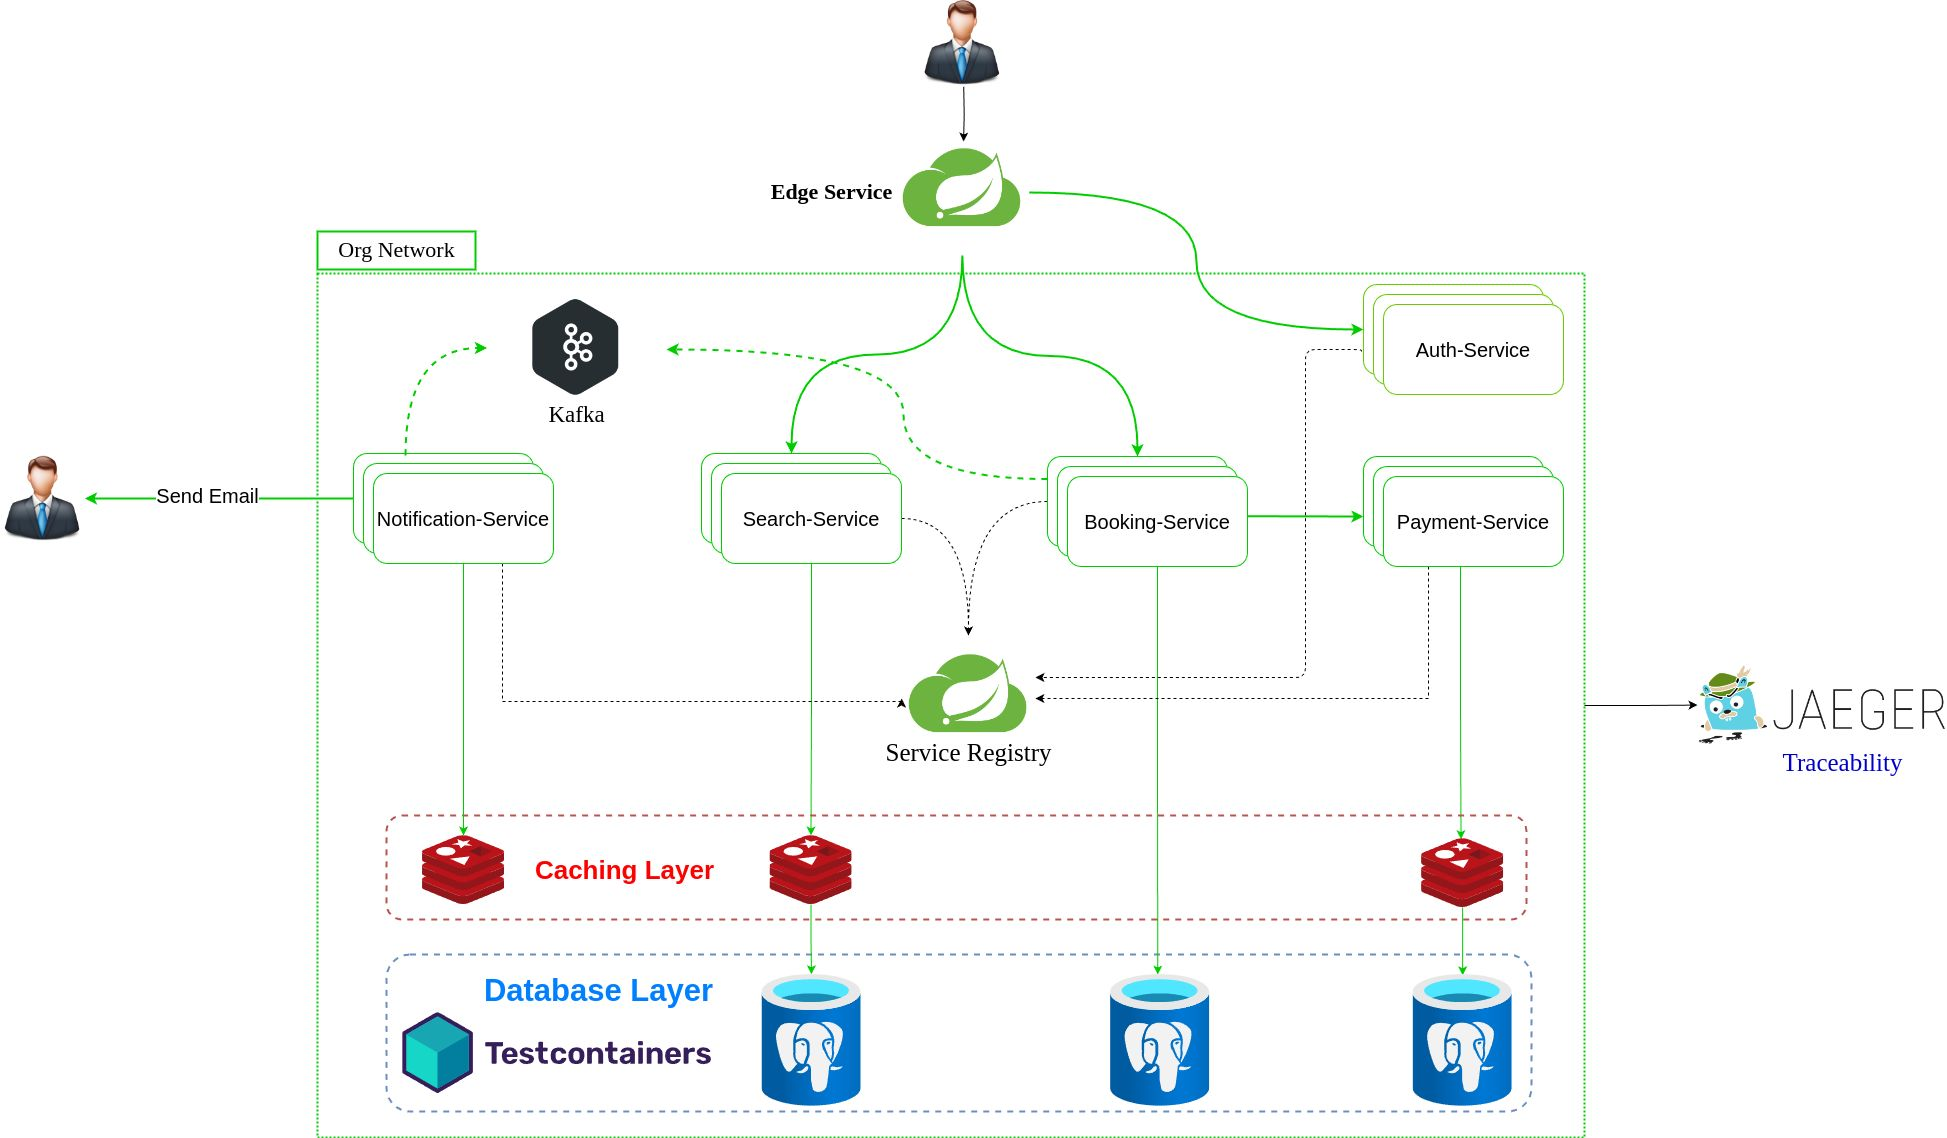
\includegraphics[width=0.99\linewidth, height=65mm, scale=1]{img/Flight-System.png}
		\end{figure}\vspace{1mm}
	\end{frame}	

	\begin{frame}
		\frametitle{Event-driven communication}
			\begin{figure}[h]
				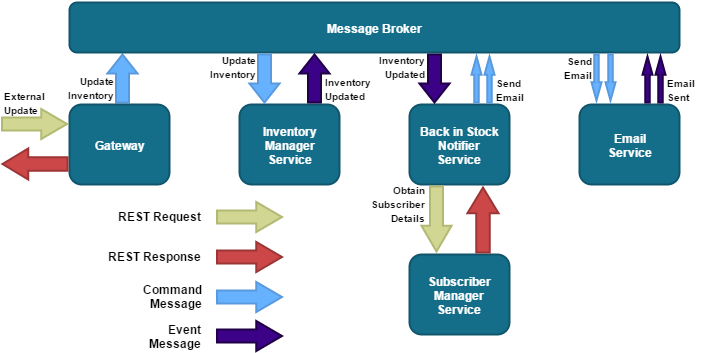
\includegraphics[width=80mm, height=50mm, scale=2]{img/mq-flow.png}
				\caption{Asynchronous calls}
			\end{figure}
		
		\vspace{5mm}
		\tiny {https://capgemini.github.io/architecture/is-rest-best-microservices}
	\end{frame}

	\begin{frame}
		\frametitle{Why not SOAP?}
				It is possible to build a microservices-based architecture using SOAP which uses HTTP. But:
			
			\vspace{5mm}
			\begin{itemize}
				\item
					\scriptsize {it only uses POST messages to transfer data to a server}.
					
				\item 
					\scriptsize{SOAP lacks concepts such as HATEOAS that enable relationships between microservices to be handled flexibly}. 
				\item 
					\scriptsize{The interfaces have to be completely defined by the server and known on the client}.
			\end{itemize}
			
			\vspace{30mm}
			\tiny {Microservices; Flexible Software Architecture. "Eberhard Wolff"}
	\end{frame}

	\subsection {API Gateway}
		\begin{frame}
		\frametitle{API Gateway}
			\scriptsize
			\begin{block} {API Gateway}
				\scriptsize {API Gateway is a tool that makes it easy for developers to create(1), publish(2), maintain(3), monitor(4), and secure(5) APIs at any scale. APIs act as the "front door" for applications to access data, business logic, or functionality from your backend services}.
			\end{block}
			\begin{figure}[h]
				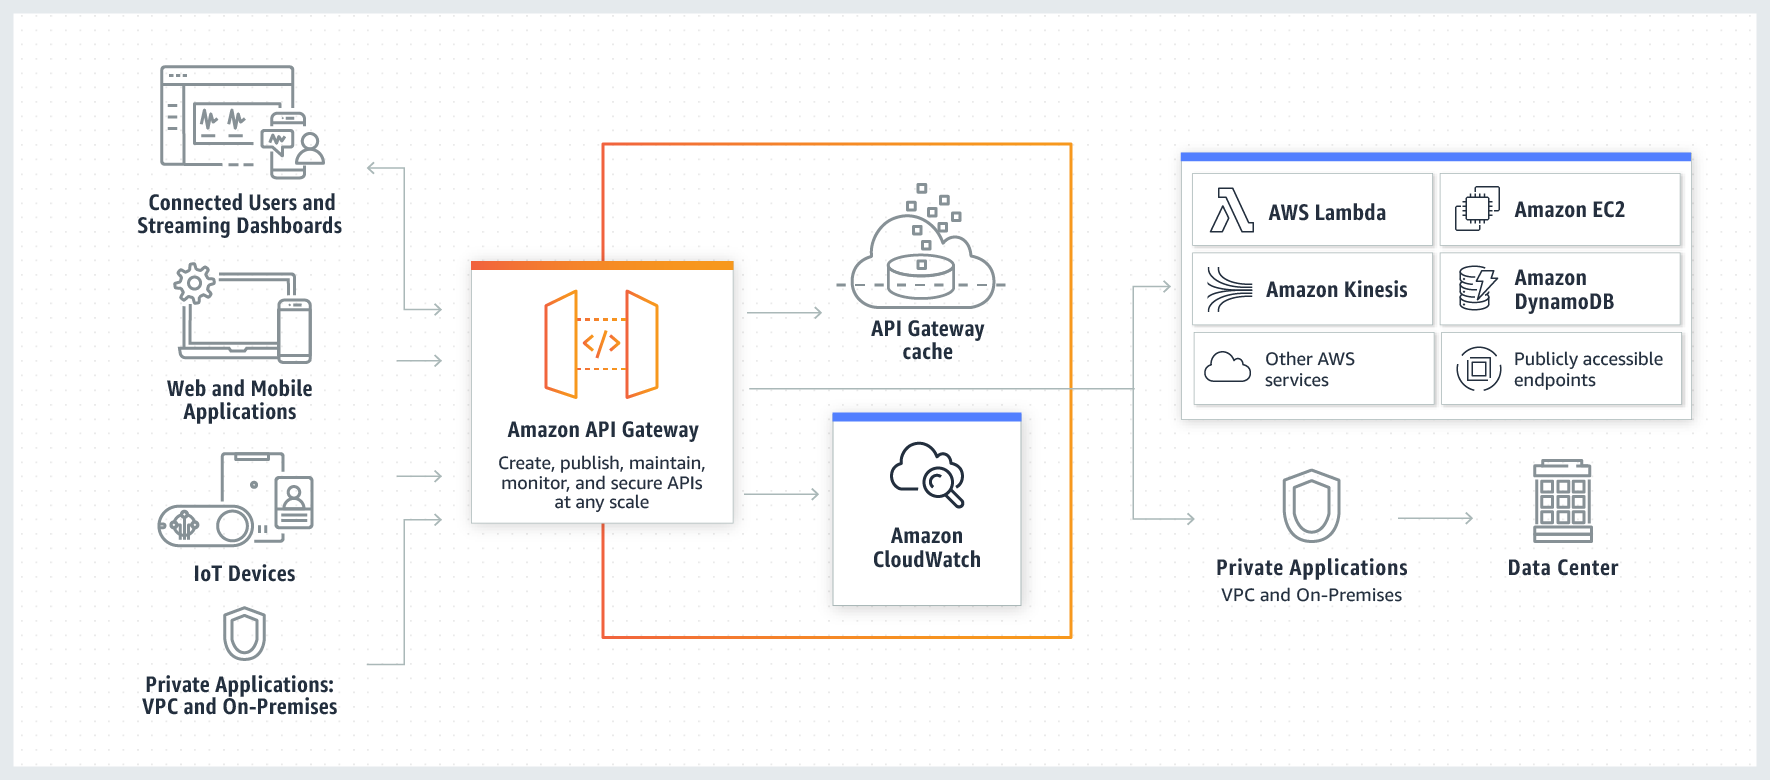
\includegraphics[width=100mm, scale=1]{img/amazon-gateway.png}
				\caption{Amazon Gateway}
			\end{figure}\vspace{1mm}
		
			\tiny{https://aws.amazon.com/api-gateway/}	
		\end{frame}
	
		\begin{frame}
			\frametitle{Orchestration and API Gateway cont...}
				\begin{figure}[h]
					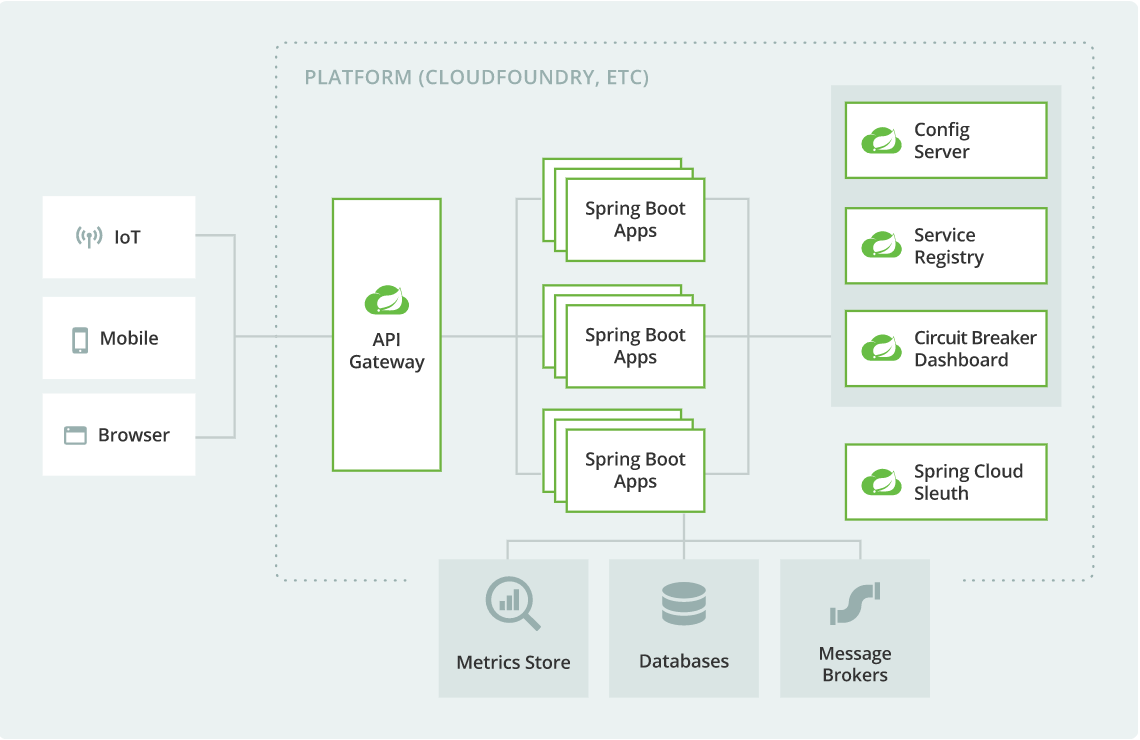
\includegraphics[width=100mm, scale=2]{img/microservice-diagrame.png}
					\caption{Microservices with Spring Cloud}
				\end{figure}\vspace{20mm}
				
				\tiny{https://spring.io/microservices}	
		\end{frame}
	
		\begin{frame}
			\frametitle{Available Market Options}
			\vspace{10mm}
				\begin{figure}[h]
					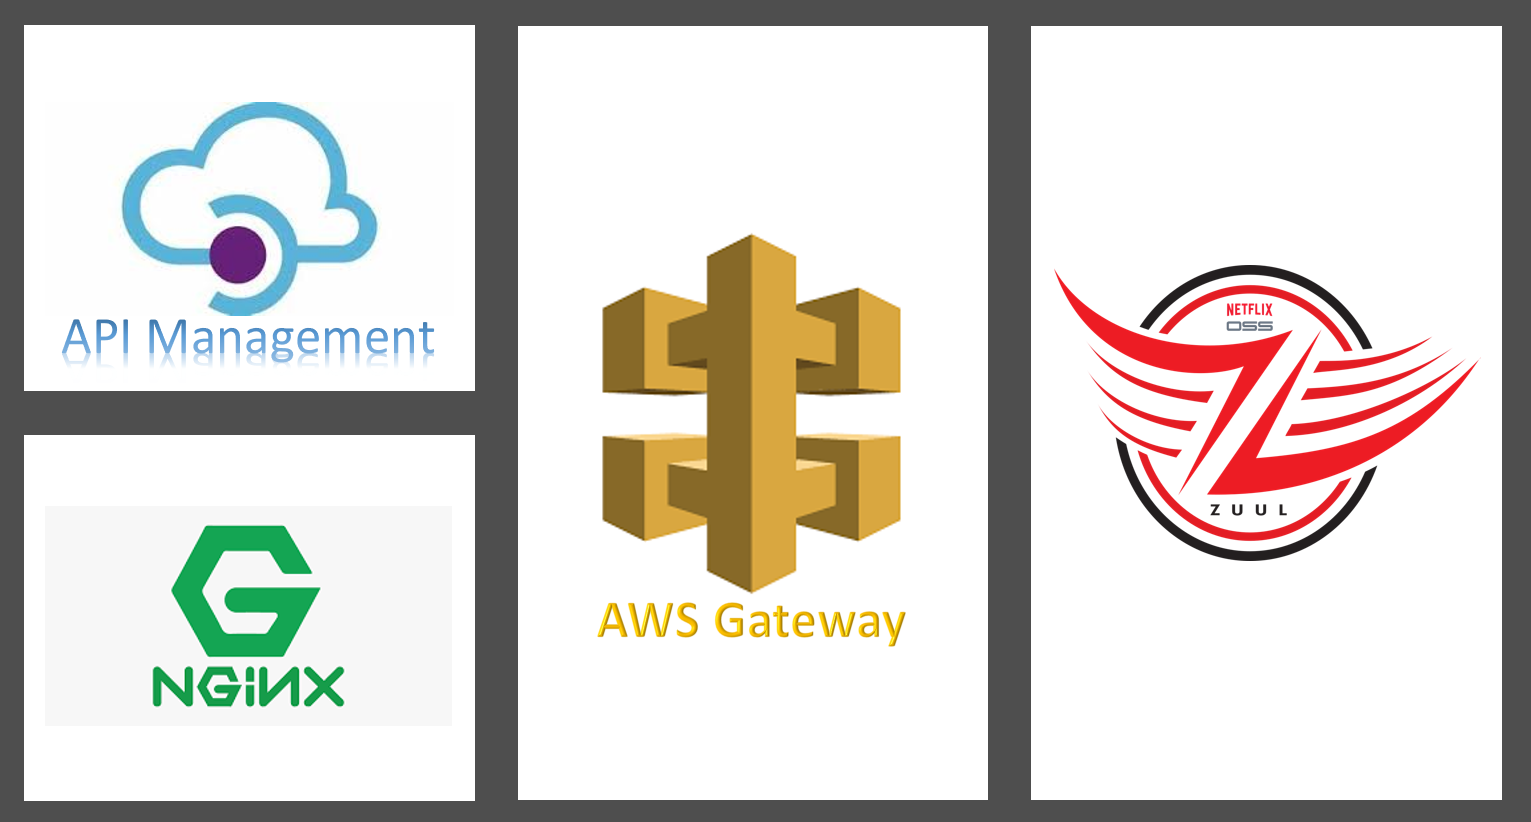
\includegraphics[width=100mm, scale=2]{img/gtws.png}
					\caption{API Gateway Products}
				\end{figure}\vspace{20mm}
			
	\end{frame}
		
	
	
	\subsection {Service Discovery}
		\begin{frame}
			\frametitle{Service Discovery}
			\scriptsize
				\textbf {Problem} \par
				In any distributed architecture, we need to find the physical address of where a machine is located.
				
				\vspace{2mm}
				\textbf {Solution} \par	
					Using service discovery, a service can register itself when it is up and healthy. By using such technology you can achieve: 
						\begin{enumerate}
							\item<1->	Load balanced
								\begin{itemize}
									\item \scriptsize {dynamically load balance requests across all service instances to ensure that the service invocations are spread across all the service instances managed by it.}
								\end{itemize}
							\item<2-> 	Resilient
								\begin{itemize}
									\item \scriptsize {client should “cache” service information locally. Local caching allows for gradual 		degradation of the service discovery feature so that if service discovery service does become unavailable, applications can still function and locate the services based on the information maintained in its local cache.}
								\end{itemize}
							\item<3->	Fault-tolerant
								\begin{itemize}
									\item \scriptsize {detect when a service instance isn’t healthy and remove the instance from the list of available services.}
								\end{itemize}
							
						\end{enumerate}
			\vspace{10mm}
			\tiny{Spring Microservices in Action, ``JOHN CARNELL``}	
		\end{frame}
		
		\begin{frame}
		\frametitle{Service Discovery with Gateway}
			\begin{figure}[h]
				\centering
				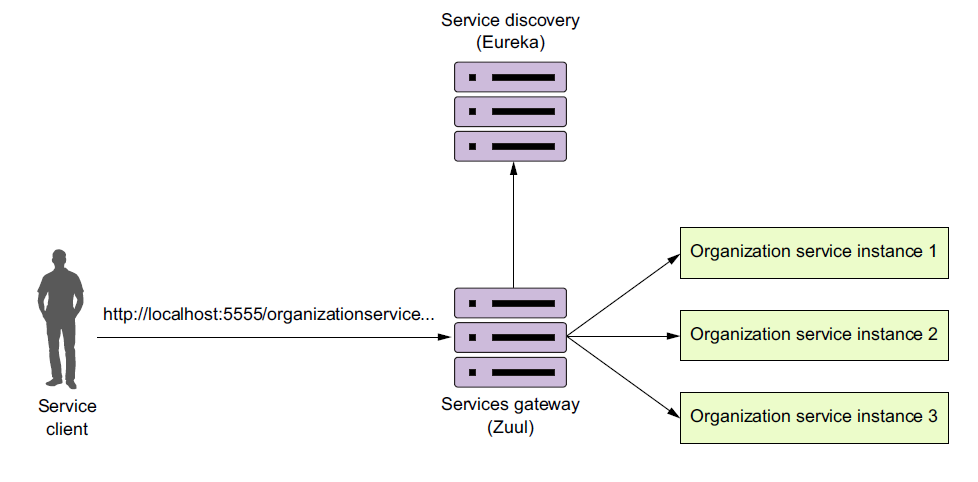
\includegraphics[width=.8\linewidth]{img/zull-and-sd.png}
				\caption{Service Registry and Gateway}
			\end{figure}
		\vspace{10mm}
		\tiny{Spring Microservices in Action, ``JOHN CARNELL``}	
		\end{frame}
		
		\begin{frame}
			\frametitle{Available Market Options}
				\begin{figure}[h]
						\centering
						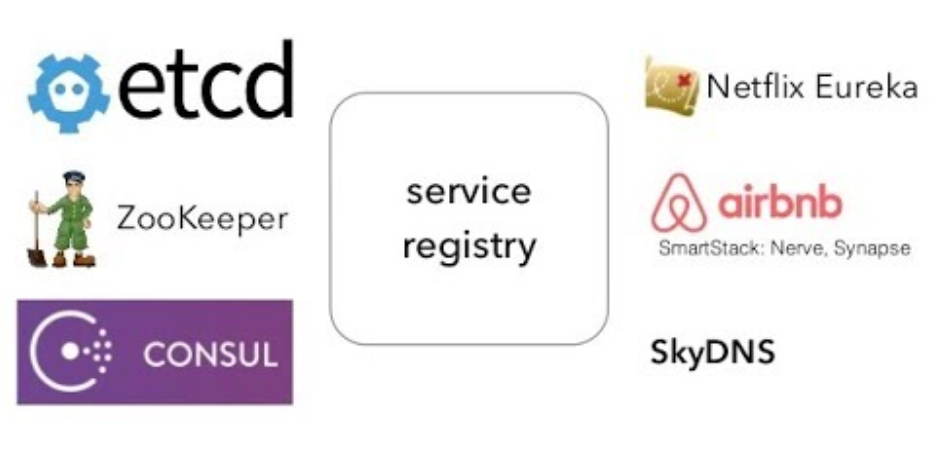
\includegraphics[width=.8\linewidth]{img/SR.png}
						\caption{Service Registry Products}
				\end{figure}
		\end{frame}

	\subsection {Externalized Configurations}
		\begin{frame}
			\frametitle{Externalized and \color{blue} {Dynamic Configurations}}
			\scriptsize
				\textbf {Problem} \par
					\hspace{3mm} Configurations will vary from environment to another, How to manage them?
				
				\vspace{2mm}
				\textbf {Solution} \par	
					\hspace{3mm} Centralize your configuration
				
				\begin{figure}[h]
					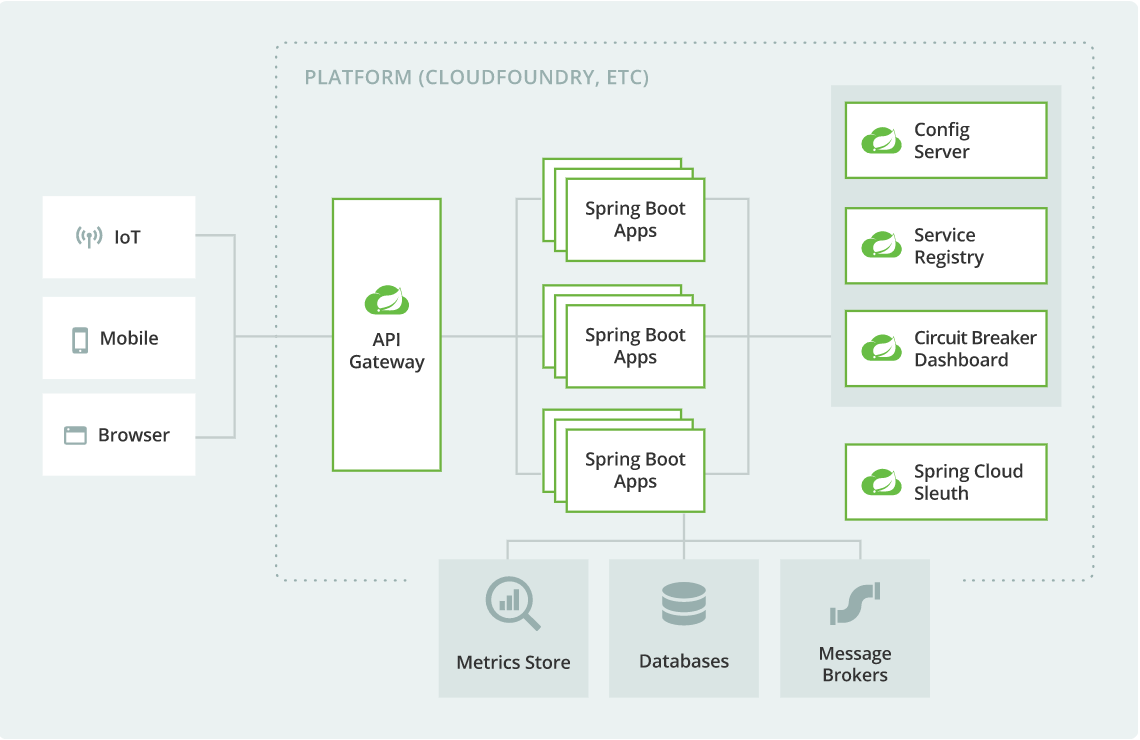
\includegraphics[width=100mm,height=50mm, scale=1]{img/microservice-diagrame.png}
					\caption{Microservices with Spring Cloud}
				\end{figure}\vspace{20mm}
				
				\tiny{https://spring.io/microservices}	
		\end{frame}
	
	\begin{frame}
		\frametitle{Available Market Options}
			
			\begin{figure}[h]
				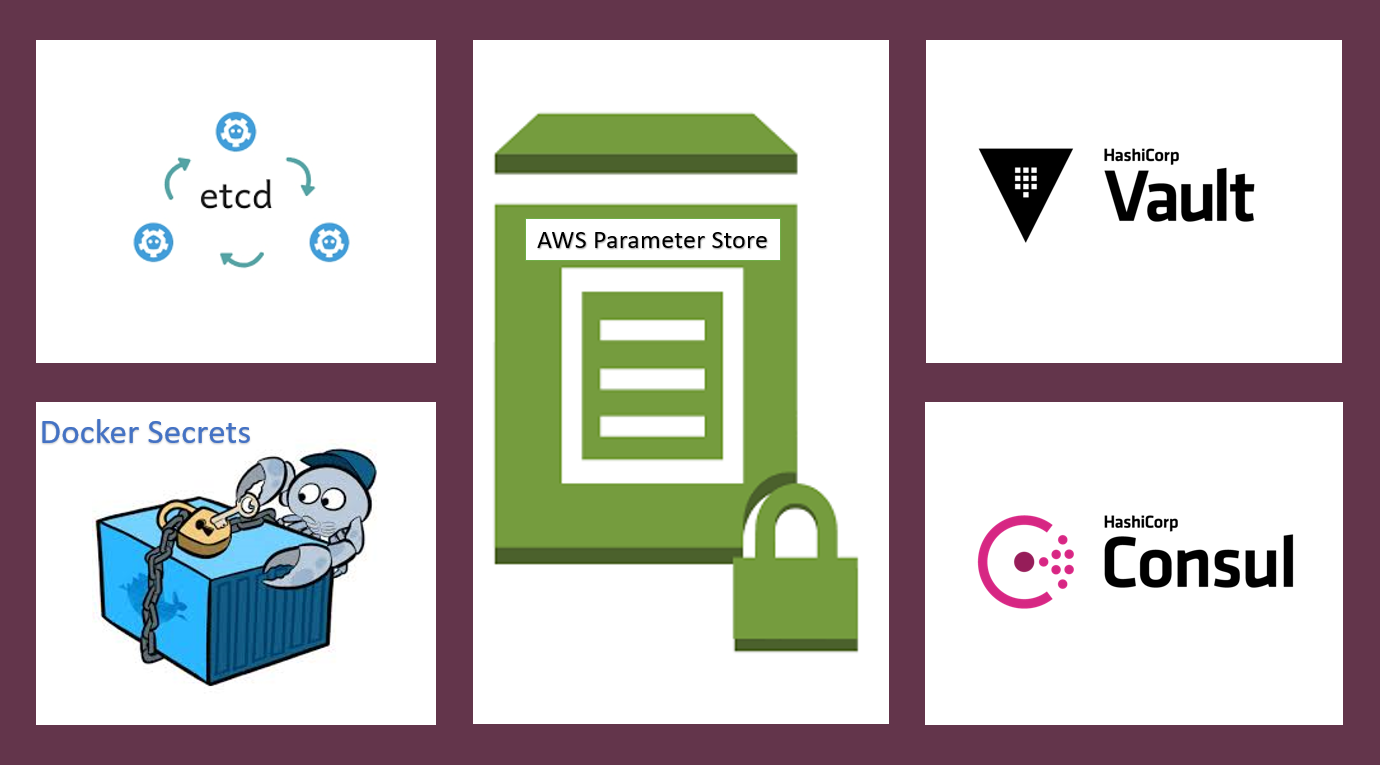
\includegraphics[width=100mm,height=60mm,  scale=1]{img/Configs.png}
				\caption{Popular Config Stores}
			\end{figure}\vspace{20mm}
			
			\tiny{https://spring.io/microservices}	
	\end{frame}

	\subsection {Circuit Breaker Pattern}
		\begin{frame}
			\frametitle{Circuit Breaker Pattern}
			\textbf {Problem} \par
			\begin{itemize}
				\item<1-> \scriptsize {One of the big differences between in-memory calls and remote calls is that remote calls can fail, or hang without a response until some timeout limit is reached}.
				\item<2-> \scriptsize {What's worse if you have many callers on a unresponsive supplier, then you can run out of critical resources leading to cascading failures across multiple systems}.
			\end{itemize}  
			\textbf {Solution} \par
			\hspace{3mm} \small {Fault Tolerance}
			\begin{figure}[h]
				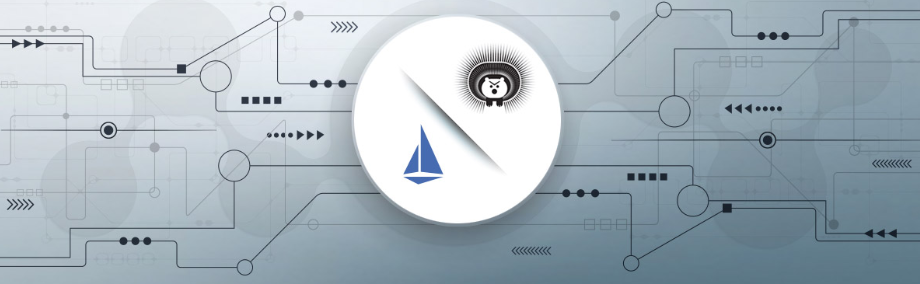
\includegraphics[width=100mm,scale=1]{img/cbp.png}
				\caption{Circuit Breaker}
			\end{figure}\vspace{20mm}
		
			\tiny{https://www.exoscale.com/syslog/istio-vs-hystrix-circuit-breaker/}	
		\end{frame}

	\subsection {Deployment and Hosting}
		\begin{frame}
			\frametitle{Service Orchestrators}
				An orchestrator handles tasks of deploying and managing a set of services. With orchestrator you can 
				\scriptsize
				\begin{itemize}
					\item<1-> Placing services on nodes. 
					\item<2-> Monitoring the health of services and restarting unhealthy services.
					\item<3-> Load balancing network traffic across service instances. 
					\item<4-> Service discovery
					\item<5-> Scaling the number of instances of a service
					\item<6->[]
						\vspace{5mm}
						\begin{columns}[c]
							\column{.30\textwidth} 
							Popular Orchestrators
							\begin{itemize}
								\item Docker Swarm
								\item Kubernates
								\item AWS ECS
								\item Service Fabric
								\item Openshift
							\end{itemize}
							
							\column{.70\textwidth} % Right column and width
							\begin{figure}[h]
								
\includegraphics[width=70mm, height=20mm, scale=1]{img/service-orch.png}
							\end{figure}\vspace{1mm}
						\end{columns}
				\end{itemize}
			\vspace{100mm}
		\end{frame}
	
		\begin{frame}
			\frametitle{Real Example}
			\textit{Continuous Integration, and Deployment are your friends}
			
			\vspace{1mm}
			
			\begin{figure}[h]
				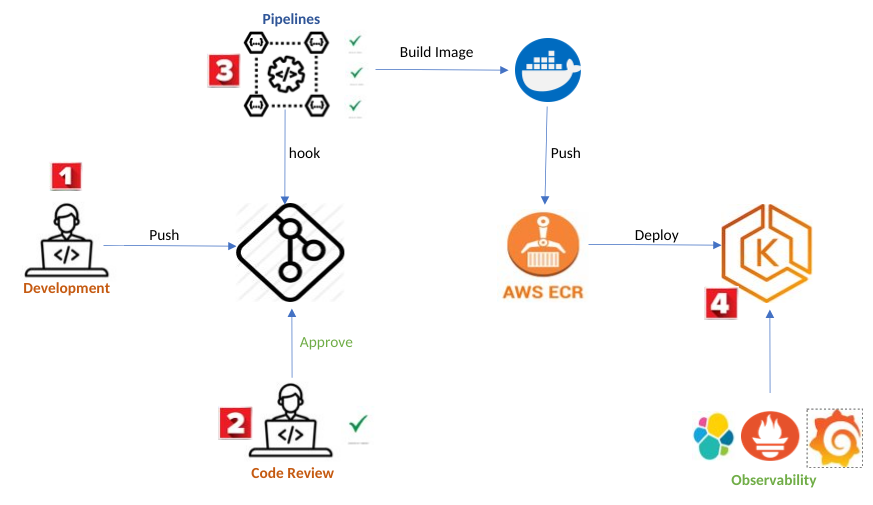
\includegraphics[width=110mm, height=60mm, scale=1]{img/all-in-one.png}
			\end{figure}\vspace{1mm}
			
		\end{frame}
	
	\begin{frame}
		\frametitle{Infrastructure as Code \textbf{"IaC"}}
		What is Infrastructure?
		\begin{itemize}
			\item<2->[] \scriptsize{The components required to operate and manage IT environments like  hardware, software, networking components, an operating system, etc.}
		\end{itemize}
	\vspace{100mm}
	\end{frame}

	\begin{frame}
		\frametitle{Infrastructure as Code \textbf{"IaC"}}
		What is Infrastructure?
		\begin{itemize}
			\item<1->[] \scriptsize{The components required to operate and manage IT environments like  hardware, software, networking components, an operating system, etc.}
		\end{itemize}
		
		Problem Statement
		\begin{itemize}
			\item<1->[] \scriptsize{Building and running servers manually using scripts or UI consoles is headache, and usually lead to configuration drift, and unexpected errors that require extra time which might not be planned!}
			\vspace{1mm}
			\item<2-> \scriptsize{The reason is Operator/SysAdmin usually uses \textbf{Imperative} way on building his job}
			\item<3-> \scriptsize{Everything should be automated and following pipelines}
			\item<4-> \scriptsize{It is better to use \textbf{Declarative} way on building such pipelines}
			\item<5-> \scriptsize{Writing declarative files (JSON, YAML or XML) can be reviewed, enhanced and  apply versioning on it like normal development}
			\item<6-> \scriptsize{IaC should be always \textbf{Idempotent} this will enable Ops team to test their work on production-like environment before actual production}
			\item<7-> \scriptsize{Should I (SysAdmin/Operator) learn programming to apply IaC?}
		\end{itemize}
	\vspace{100mm}
	\end{frame}

	\begin{frame}
		\frametitle{Infrastructure as Code \textbf{"IaC"}}
			\begin{figure}[h]
				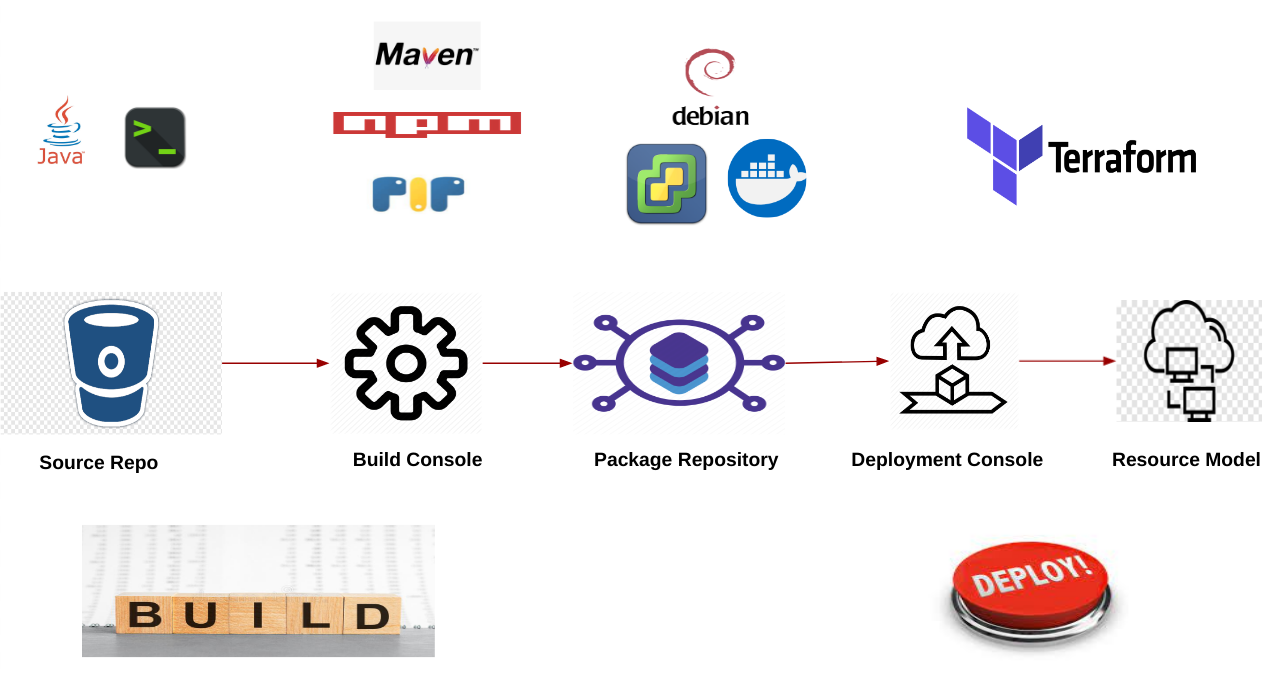
\includegraphics[width=100mm,height= 70mm, scale=1]{img/service-delivery-platform.png}
				\caption{Service Delivery Platform}
			\end{figure}
	\end{frame}


	\begin{frame}
		\frametitle{Infrastructure as Code \textbf{"IaC"}}
		\begin{itemize}
			\item<1-> \scriptsize{\alert{But how to ensure quality of \textbf{code}?}}
			\item<2-> \scriptsize{Answer: \textbf{Testing}}
			\item<3-> \scriptsize{Techniques used in normal development should be applied, e.g Unit \& Integration Test}. 
				\begin{itemize} 
					\item \scriptsize{\textbf{Rubocop} Formatter and \textbf{Foodcritic} Linter}
					\item \scriptsize{\textbf{ChefSpec} Test Simulator and Coverage}
					\item \scriptsize{\textbf{ServerSpec} and \textbf{TestInfra} for Integration testing}
				\end{itemize}
			\item<4-> \scriptsize{The output of Build phase is the deliverable (Binaries), once it is created, should never be changed; this is called \textbf{Immutable Deployment}}
			\item<5-> \scriptsize{There will be always kind of tension between Dev team and Ops team; especially if Ops team is applying SRE principles}
			\item<1->[]
			\begin{figure}[h]
				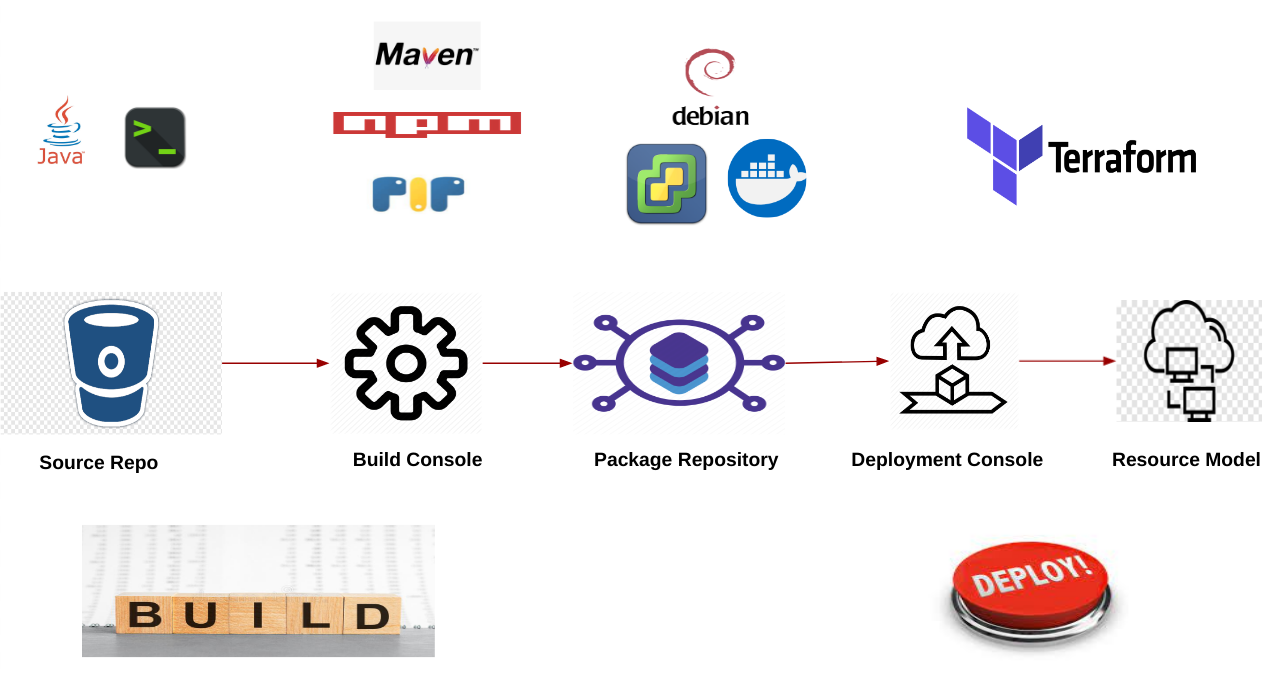
\includegraphics[width=100mm,height= 47mm, scale=1]{img/service-delivery-platform.png}
				\caption{Service Delivery Platform}
			\end{figure}
		\end{itemize}
	\end{frame}
	
	\againframe{cd}
	
	
	\begin{frame}
		\frametitle{Communication Design - Async \& Messaging}
		Online purchase example
		\scriptsize
		\begin{itemize}
			\item<2-> Save it
			\item<3-> Check Duplicates
			\item<4-> Charge Customer
			\item<5-> Send Email to customer
			\item<6-> Audit Order details 
		\end{itemize}
	\vspace{100mm}
	\end{frame}

	\begin{frame}
		\frametitle{Communication Design - Async \& Messaging}
		
		\begin{figure}[h]
			\includegraphics[width=100mm,height= 70mm, scale=1]{img/kafka-architecture.png}
		\end{figure}
		\vspace{100mm}
	\end{frame}

	
	\begin{frame}
		\frametitle{Scalability and High Availability}
		Scalability is about your system capability to scale (In or Out) in order to handle workload and throughput
		\begin{itemize}
			\item<2-> Vertical Scaling
				\begin{itemize} 
					\item<3-> \scriptsize{Database scaling for example by adding more CPU and Memory power} 
					\item<4-> \scriptsize{Cons: \alert {Can't work in all cases, expensive} }
				\end{itemize}
			\item<5-> Horizontal Scaling
				\begin{itemize} 
					\item<6-> \scriptsize{Increase numbers of workers, with same power capacity} 
					\item<7-> \scriptsize{Good choice for distributed systems}
					\item<8-> \scriptsize{Cons: \alert {Network Latency and Management Complexity} }
				\end{itemize}
		
			\item<9-> High Availability
			\begin{itemize} 
				\item<10-> \scriptsize{The availablity percentage of your service within period of time} 
				\item<11-> \scriptsize{SLA is 99.99\%}
			\end{itemize}
		
		\end{itemize}
		\vspace{100mm}
	\end{frame}


	\begin{frame}
		\frametitle{Scalability and High Availability}
		\begin{figure}[h]
			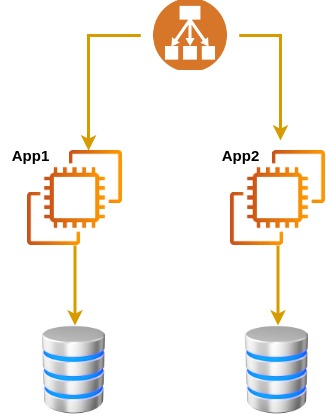
\includegraphics[width=50mm, height=50mm, scale=1]{img/Scalability-1.jpg}
		\end{figure}	
	\end{frame}

	\begin{frame}
		Horizontal Scaling
		\frametitle{Scalability and High Availability}
		\begin{figure}[h]
			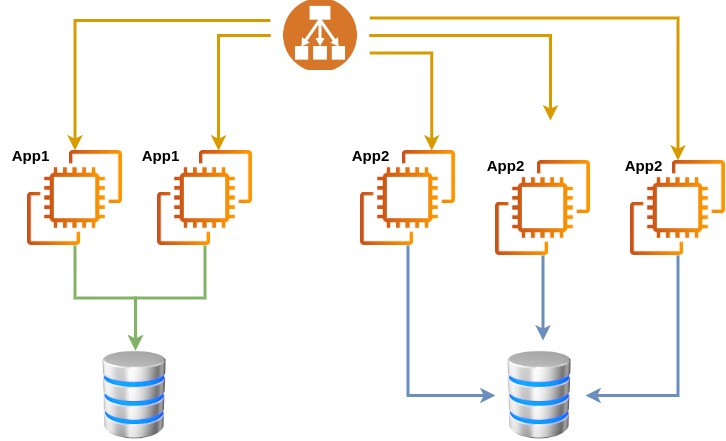
\includegraphics[width=70mm, height=50mm, scale=1]{img/horizontal-scaling.jpg}
		\end{figure}	
	\end{frame}

	\begin{frame}
		\frametitle{Scalability and High Availability}
		Fault Tolerant
		\begin{figure}[h]
			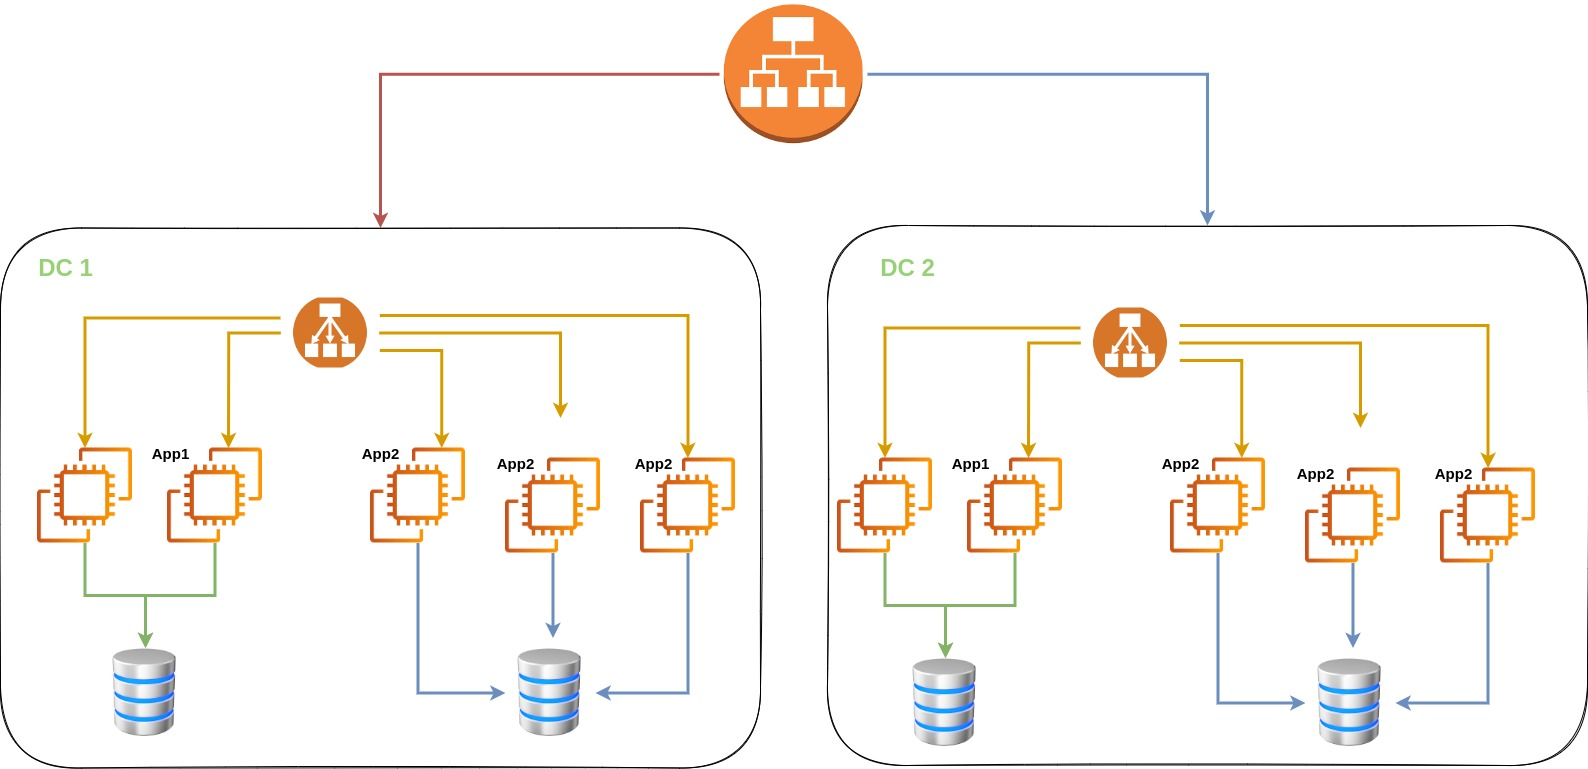
\includegraphics[width=100mm, height=70mm, scale=1]{img/High-Availability.jpg}
		\end{figure}	
	\end{frame}	

	
\begin{frame}
\frametitle{References}
\footnotesize{
\begin{thebibliography}{99} % Beamer does not support BibTeX so references must be inserted manually as below
	\bibitem[Eric Evans, 2003]{p1} Eric Evans, (2003)
	\newblock Domain-Driven Design: Tackling Complexity in the Heart of Software
\end{thebibliography}
}
\end{frame}

%------------------------------------------------

\begin{frame}
\Huge{\centerline{Thank You}}
\end{frame}

%----------------------------------------------------------------------------------------

\end{document} 